%!TEX root =  ../main.tex

\subsection{Numerical, Graphical, Algebraic, and Verbal}


\objective{Use functions defined numerically, graphically, algebraically, or verbally.}



A \gls{function} is a relation that uniquely associates members of one \gls{set} 
with members of another set.  
More simply, a function connects members of a \gls{domain} to members of a \gls{range}, 
with the proviso that each element in the domain maps onto only one element in the range.  
When graphing a function, it is customary to plot the \emph{input} or \gls{independent variable} 
on the $x$-axis (going left to right), and the \emph{output} or \gls{dependent variable} on 
the $y$-axis (going down to up).  The independent variable is so-called because it may 
be arbitrarily chosen from within the domain.  The dependent 
variable is then forced to be a particular value (by the function).

\subsubsection{Numerically}
Typically, information is gathered about the physical world as \gls{discrete} numbers, 
occurring at fixed points. Such information may be represented as in table~\ref{tab:Numerically}.

\columntable[-0.75in]{1.6in}{
  \begin{tabular}{ lr }
  \hline
  \textbf{x} (months since) & \textbf{y} (100's of \$)\\
  \hline
  0 & 1200.00 \\
  1 & 840.00 \\
  10 & 1680.24 \\
  16 & 2072.98 \\
  23 & 2264.72 \\
  36 & 4303.93 \\
  48 & 6770.53 \\
  \hline
  \end{tabular}
   }{Monthly income represented numerically\label{tab:Numerically}}
    
    
\subsubsection{Graphical}
A helpful way to visualize relationships between input and output 
sets is a \gls{graph} of the function.  Similar techniques
include diagrams (see Figure for an example) and maps (see Figure for an example).  
``Mapping diagrams'' blur the line between numerical and graphical data 
(see Figure ~\ref{fig:graphically} for an example).

\begin{figure}[h]
\centering
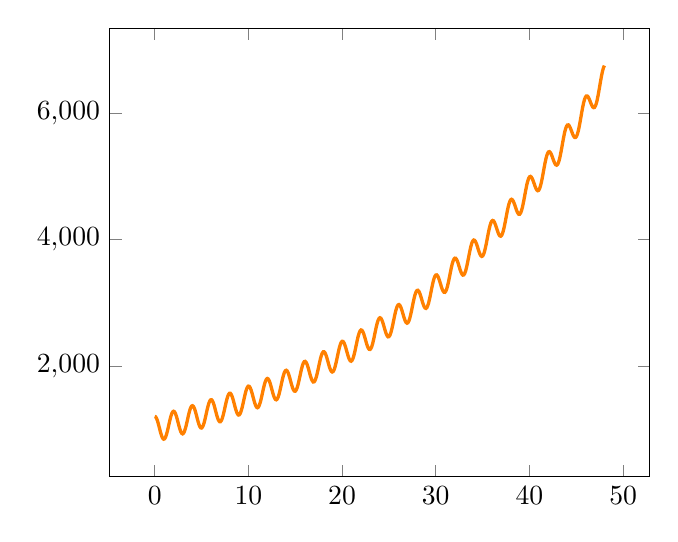
\begin{tikzpicture}
\begin{axis}[samples=500,domain=0:48,restrict y to domain =0:8500]
\addplot[very thick,orange ]plot (\x, {1000*(pow(1.04,\x))+200*cos((\x r)*3.1415)});
\end{axis}
\end{tikzpicture}
\caption[Graph]{Monthly Income  - Graphically\label{fig:graphically}}
\end{figure}


\subsubsection{Algebraically}
Typically, graphs come from humans or machines plotting many, 
many points derived from an \gls{algebraic} formula.
Algebra is a powerful tool for describing natural phenomena, 
but it cannot do everything.  Important numbers
--- such as \gls{pi} or $e$ --- cannot be defined via algebraic techniques.  
Worse, many confuse manipulation of the symbols with actual mathematics.
However, the symbols are very concise, as you might see in Tab.~\ref{tab:algebra}.

\columntable[-0.75in]{0.3in}{
\begin{center}
$y=1000\cdot1.04^x+200\cos(\pi x)$.
\end{center}}
{Monthly Income - Algebraically\label{tab:algebra}}



\subsubsection{Verbally}
Ordinary language serves us well most of the time, with an average level of 
precision and an average level of
emotional content.  Sometimes, however, what we wish to convey is more 
meaningful and deep than
regular wording can describe.  Conversely, we might wish to exclude a whole 
host of meanings, and narrowly
zoom in on precise terminology, in order to avoid error to the fullest extent possible
(see Fig.~\ref{fig:lol}).

\marginfig[-0in]{\chapdir/pics/levelsoflanguage}{Levels of language\label{fig:lol}}

Most of us encounter poetic language\index{language} in the form of songs, since ours is an 
age sadly bereft of
poetry, something that was not true a century ago or more.  Another common 
phenomenon is to meet 
technical language when it is not expected or welcome, such as when we read the 
instruction manual for new
hardware or legal documents.  However, such documents are typically not aiming at 
easy comprehension, but
precision.  Like most jargon, they tend to use mostly ordinary words in extraordinary 
ways, similar but opposite
to poetry.

Mathematics is no different.  This textbook is a formal setting, and as such, 
it uses technical language, carefully
choosing each word according the conventions and definitions ``in house''.  
As you cross the threshold into the
beginning stages of advanced mathematics, you must cultivate the skill of 
using this ``jargon'', something you 
do not ordinarily do.  It may help your comprehension to paraphrase 
what you are learning into the ``vernacular,''
but you should not consider a topic concluded until you are able to 
re-articulate the mater in mathematical terminology.
For example, the equation above might be described as in Fig.~\ref{fig:verbally}.

\begin{figure}
\emph{The income ($y$) may be modeled by the number of months since 
inception ($x$) as a sinusoid with an amplitude of 200, a period of 2, and a
midline of an exponential growth rate of 4\% beginning at \$1,000.}
\caption{Monthly Income - Verbally\label{fig:verbally}}
\end{figure}

\subsubsection{Mathematical Models}
Functions that can be used to make predictions and 
interpretations of real-world phenomena are called \textbf{mathematical
models}.
It is important to be clear which variable is being used as input 
and which is output, so that a meaningful
relationship between independent and dependent variables 
can be ascertained.  In the model of income above,
time does not depend upon money, but rather money upon time.  
The domain of the function is the initial time
index of zero until four years later, so in months $0\le x \le 48$.  
The income varies from as low as \$840 but
generally goes up from there, so the range is $y\ge840$.

\begin{example}
	\exProblem
There are only so many hours in a day.  If you decide to stay up \emph{all} night studying, 
you will surely get
a bad grade on the test tomorrow, due to sleep deprivation.  
Sketch a reasonable graph showing hours spent sleep the day before
a test and the grade you will get on said test.  Give the domain and range of the function.

	\exSolution
One cannot possibly get less than zero hours of sleep, and presumedly around 
12 or so hours of sleep is
long enough to have slept through the exam and angered one's parents!  
Test scores are typically measured in percents, ranging from 0 to 100.

\marginfig[-1.8in]{\chapdir/pics/sleep.png}{Possible graph of sleep vs. grade}
\end{example}

~\vfill